\subsection{Resultate}

Praxisruf wurde wie in Kapitel 5 beschrieben erweitert.
Es wurde eine native iOS App entwickelt, welche den Funktionsumgang des bestehenden Mobile Clients vollständig unterstützt.
Weiter wurde mit AWS Polly ein Sprachsynthese Provider an das System angebunden.
Diese Anbindung wird verwendet, um bei Bedarf den Inhalt empfangener Benachrichtigungen automatisch vorlesen zu lassen.
Letztlich wurde WebRTC verwendet, um eine konfigurierbare Gegensprechanalge zu implementieren.
Sowohl das Vorlesen von Benachrichtigungen, als auch die Gegensprechanlage sind über das Admin UI konfigurierbar.

\subsubsection{Systemarchitektur}

Die Systemarchitektur von Praxisruf wurde im Rahmen dieses Projektes erweitert.
Betroffen davon sind der Mobile Client und Cloudservice.
Der Mobile Client wurde durch einen neuen nativen Mobile Client ersetzt.
Der Cloudservice wurde um Komponenten zur Abfrage von Sprachdaten und Signalaustausch erweitert.
Im Rahmen dieses Projektes wurde zudem der interne Aufbau des Cloudservices überarbeitet.
Der Cloudservice wird nach wie vor als einzelner Service betrieben.
Dieser Service ist aber neu in mehrere domänenspezifische Module aufgeteilt.\footnote{Siehe Kapitel 5.1}
Diese Module können in Zukunft mit wenig Aufwand aus dem monolithischen Service ausgelöst und als eigene Services betrieben werden.

\clearpage

\subsubsection{Nativer Mobile Client}

Dieses Kapitel zeigt die umgesetzten Ansichten des Mobile Clients.

\subsubsection*{Anmeldung und Konfiguration}

Der Mobile Client bietet eine einfaches Verfahren zur Anmeldung und Konfiguration.
In einem ersten Schritt gibt der Praxismitarbeitende Benutzername und Passwort ein.
Anschliessend kann er auf einer zweiten Ansicht, die gewünschte Zimmerkonfiguration wählen.
Benutzer und Zimmerkonfiguration werden dabei gespeichert.
Bis sich der Benutzer manuell abmeldet wird bei allen zukünftigen Starts der App die gespeicherte Kombination von Benutzer und Zimmerkonfiguration wiederverwendet.

\begin{figure}[h]
    \centering
    \begin{minipage}[b]{0.4\textwidth}
        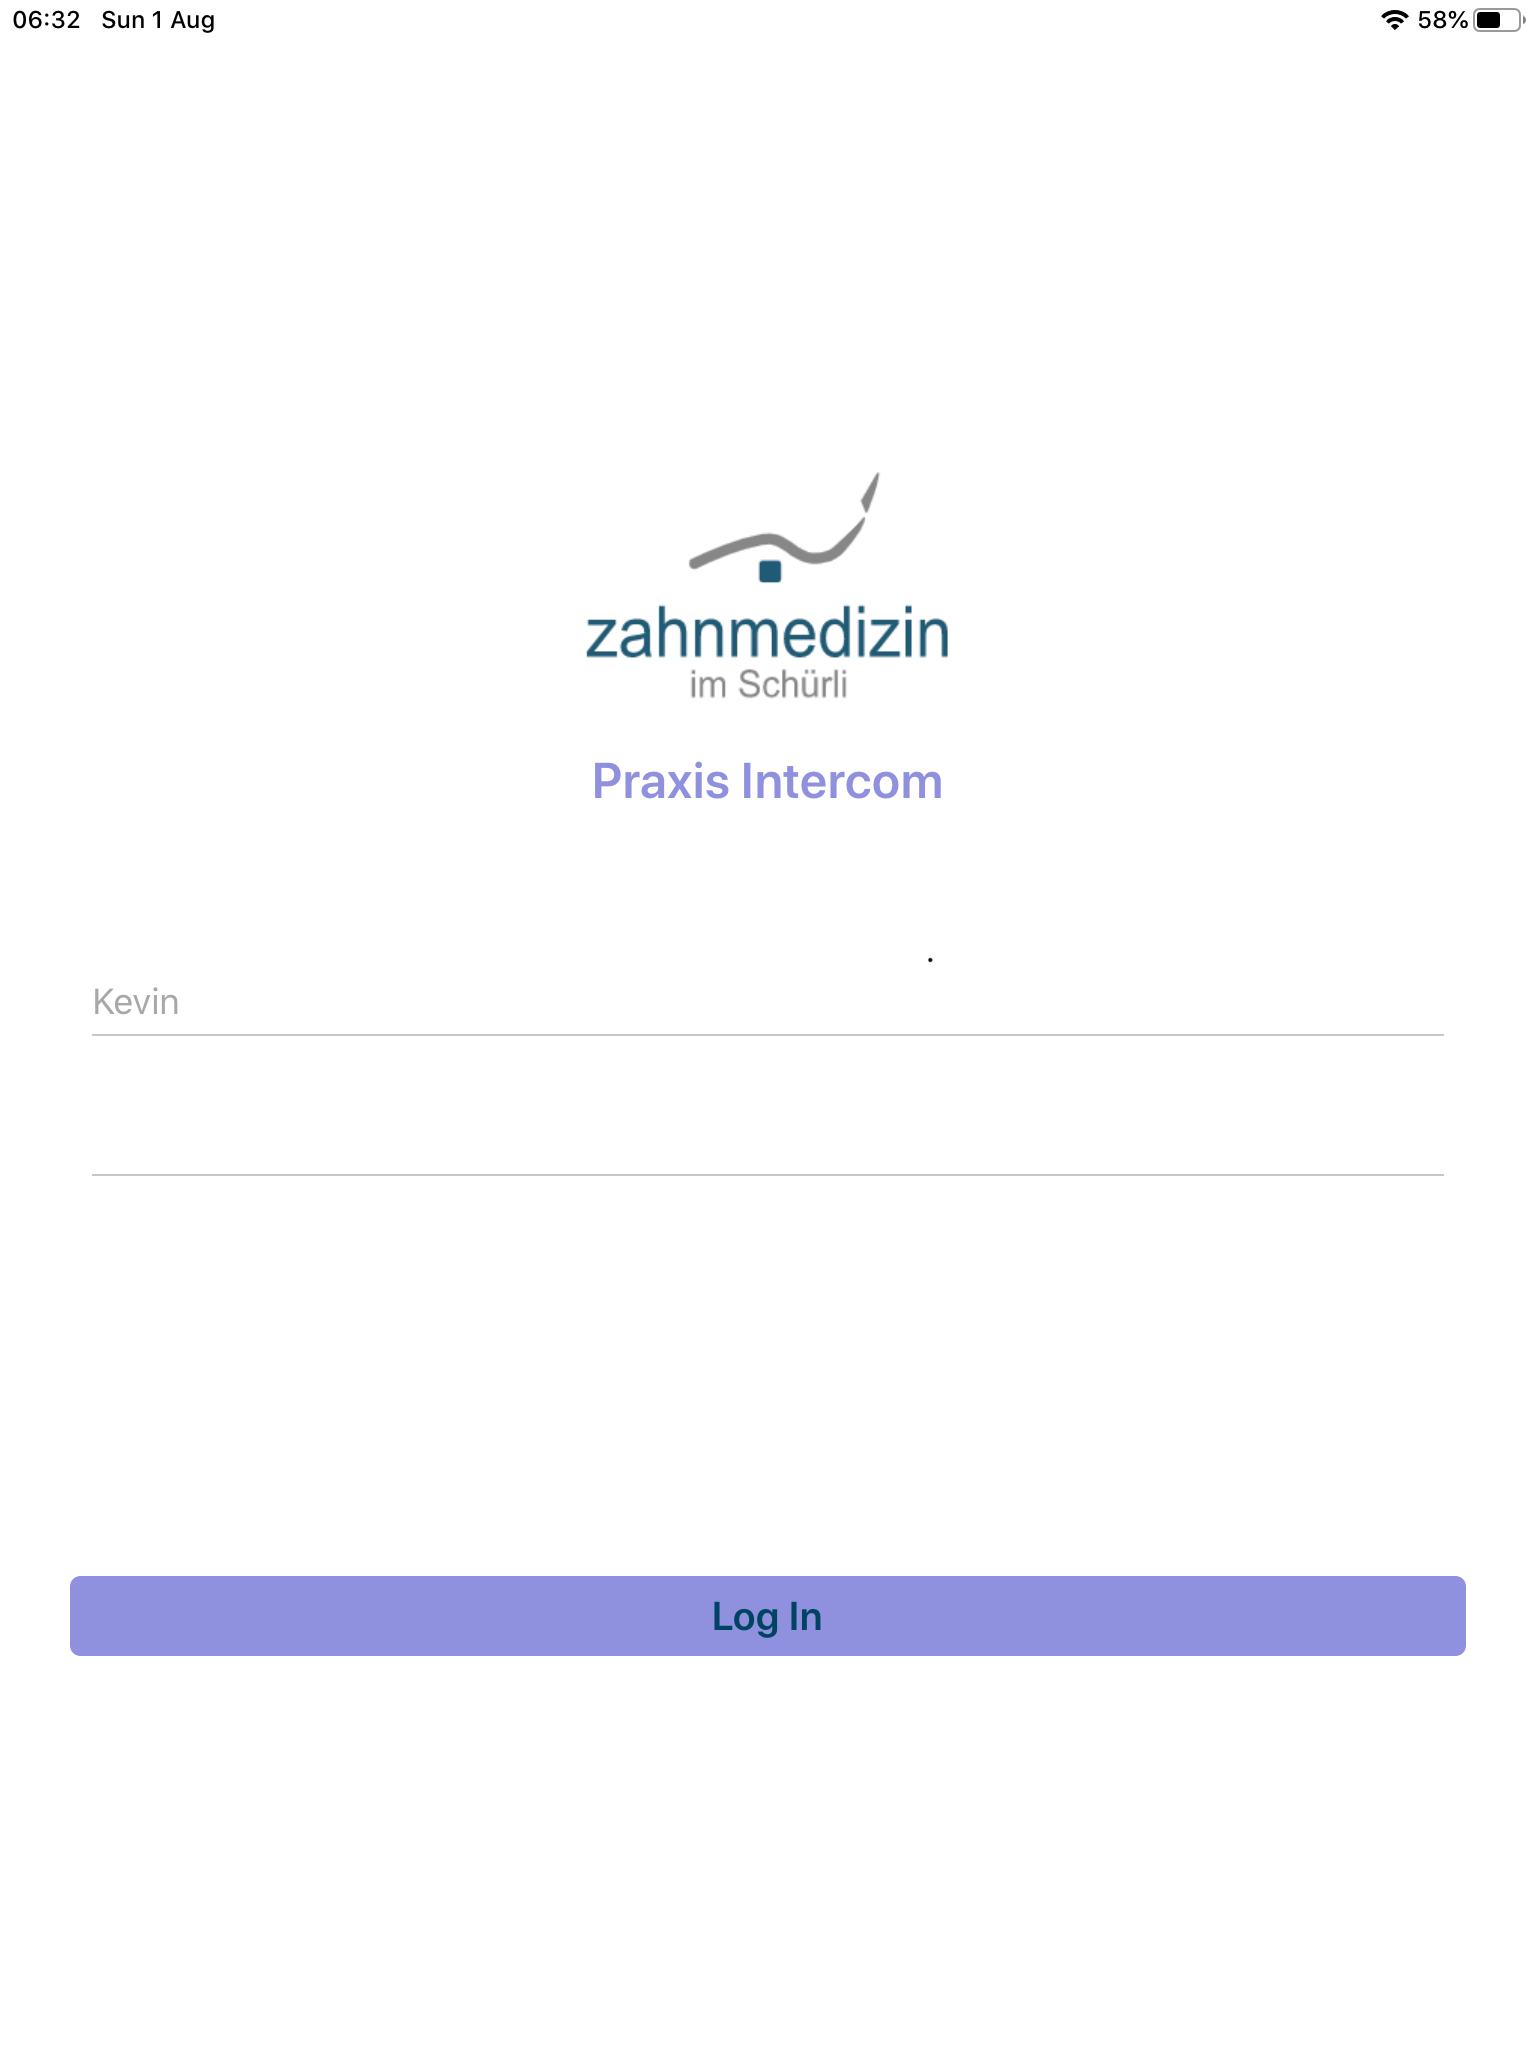
\includegraphics[width=\textwidth]{graphics/screenshots/placeholder}
        \caption{Ansicht Login}
    \end{minipage}
    \hfill
    \begin{minipage}[b]{0.4\textwidth}
        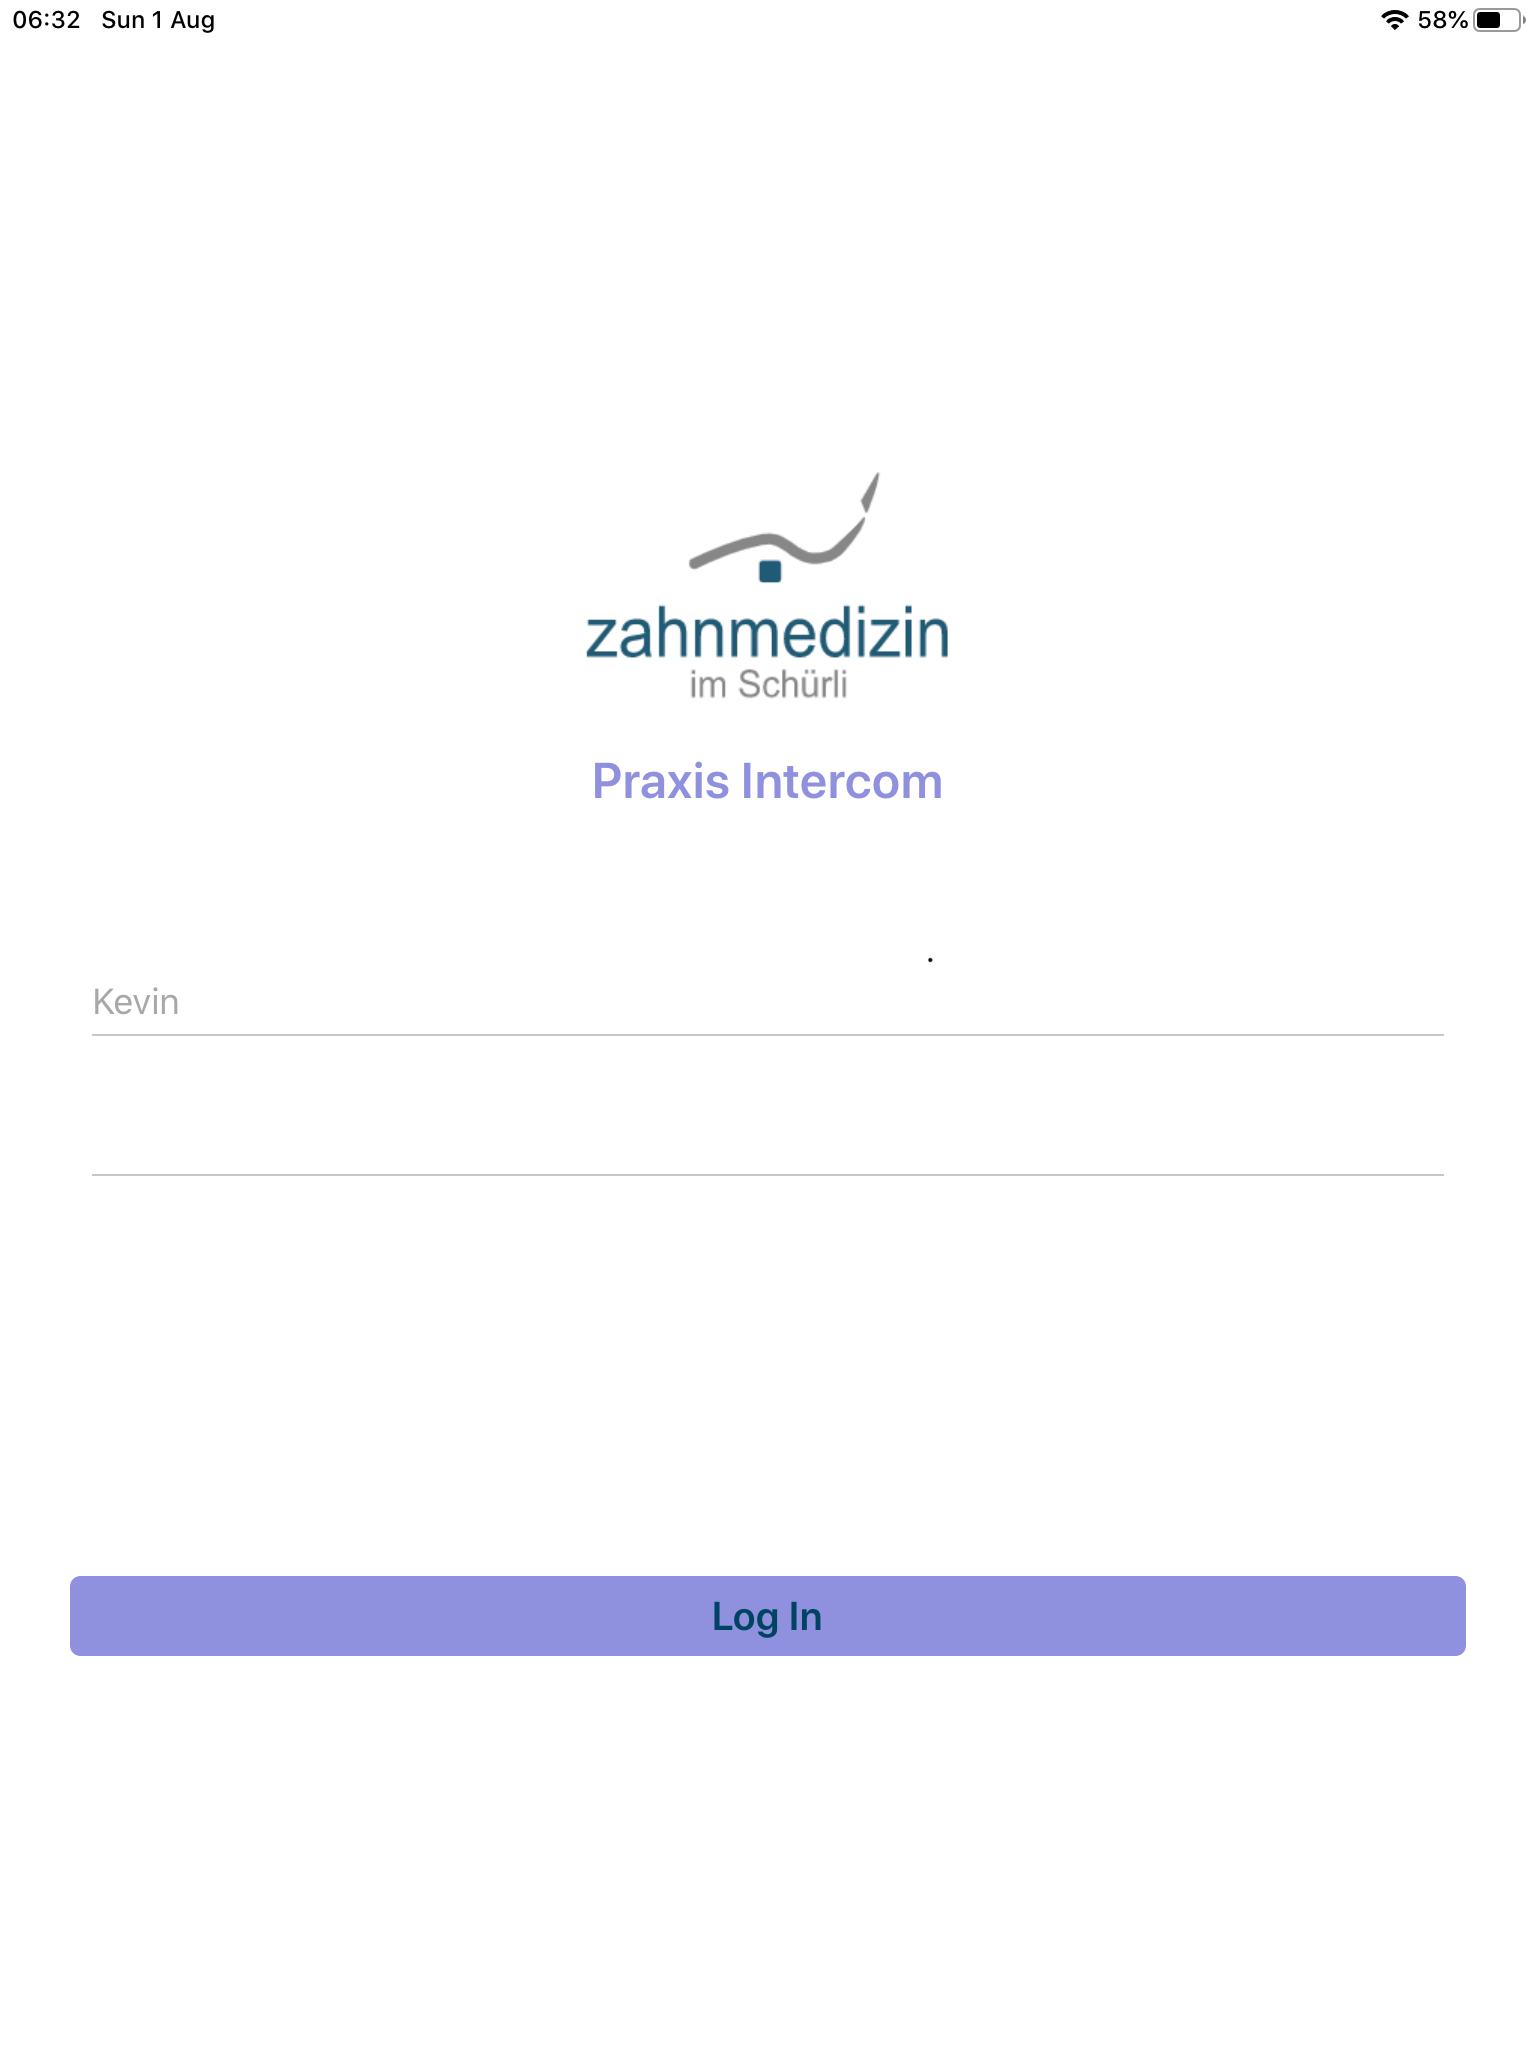
\includegraphics[width=\textwidth]{graphics/screenshots/placeholder}
        \caption{Ansicht Zimmerkonfiguration}
    \end{minipage}
    \label{fig:MobileClient-Screens1}
\end{figure}

\clearpage

\subsubsection*{Startseite und Inbox}

Nach der Anmeldung und Konfigurationsauswahl wird der Benutzer auf die Hauptansicht der App weitergeleitet.
Über eine Navigationsleiste am unteren Bildschirmrand kann zwischen den Bereichen Home, Inbox und Einstellungen
Der Bereich Home ist in zwei Teile gegliedert und beinhaltet Buttons über welche Benachrichtigungen versendet und Sprachverbindungen gestartet werden können.
Welche Buttons zur Verfügung stehen werden durch die gewählte Zimmerkonfiguration vorgegeben und wurden im Vorfeld vom Praxisadministrator konfiguriert.
Der Bereich Inbox zeigt eine Liste von empfangenen Benachrichtigungen sowie verpassten und vergangenen Anrufen.
Einträge in dieser Liste können durch eine Wischgeste (Swipe right) entfernt werden.

\begin{figure}[h]
    \centering
    \begin{minipage}[b]{0.4\textwidth}
        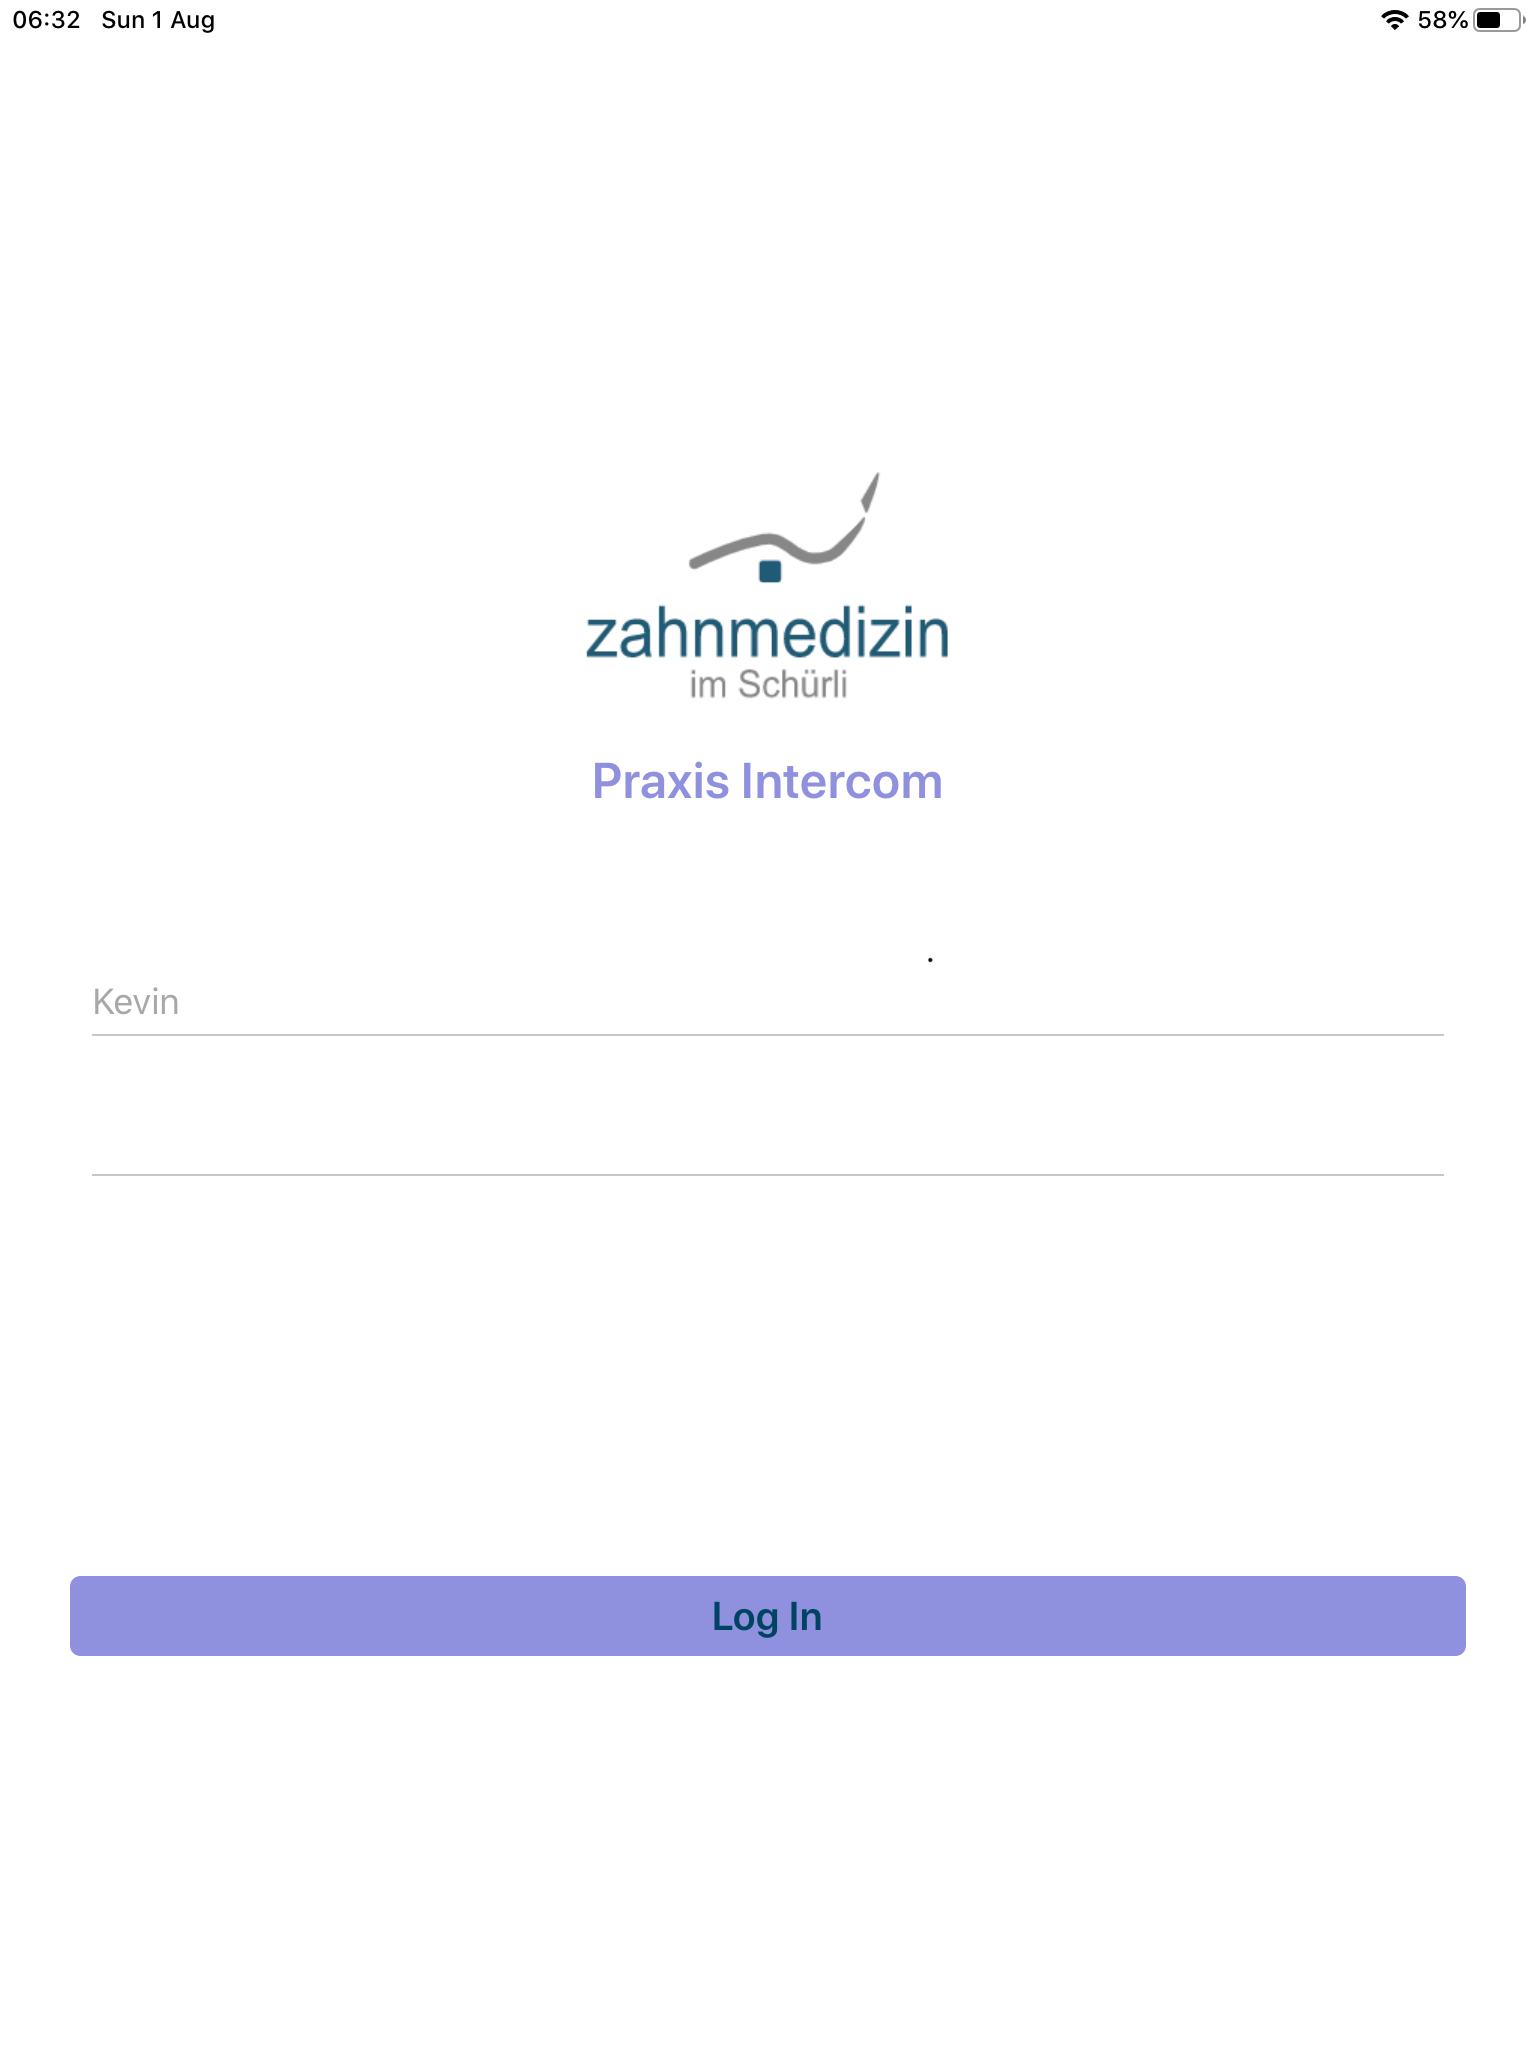
\includegraphics[width=\textwidth]{graphics/screenshots/placeholder}
        \caption{Ansicht Home}
    \end{minipage}
    \hfill
    \begin{minipage}[b]{0.4\textwidth}
        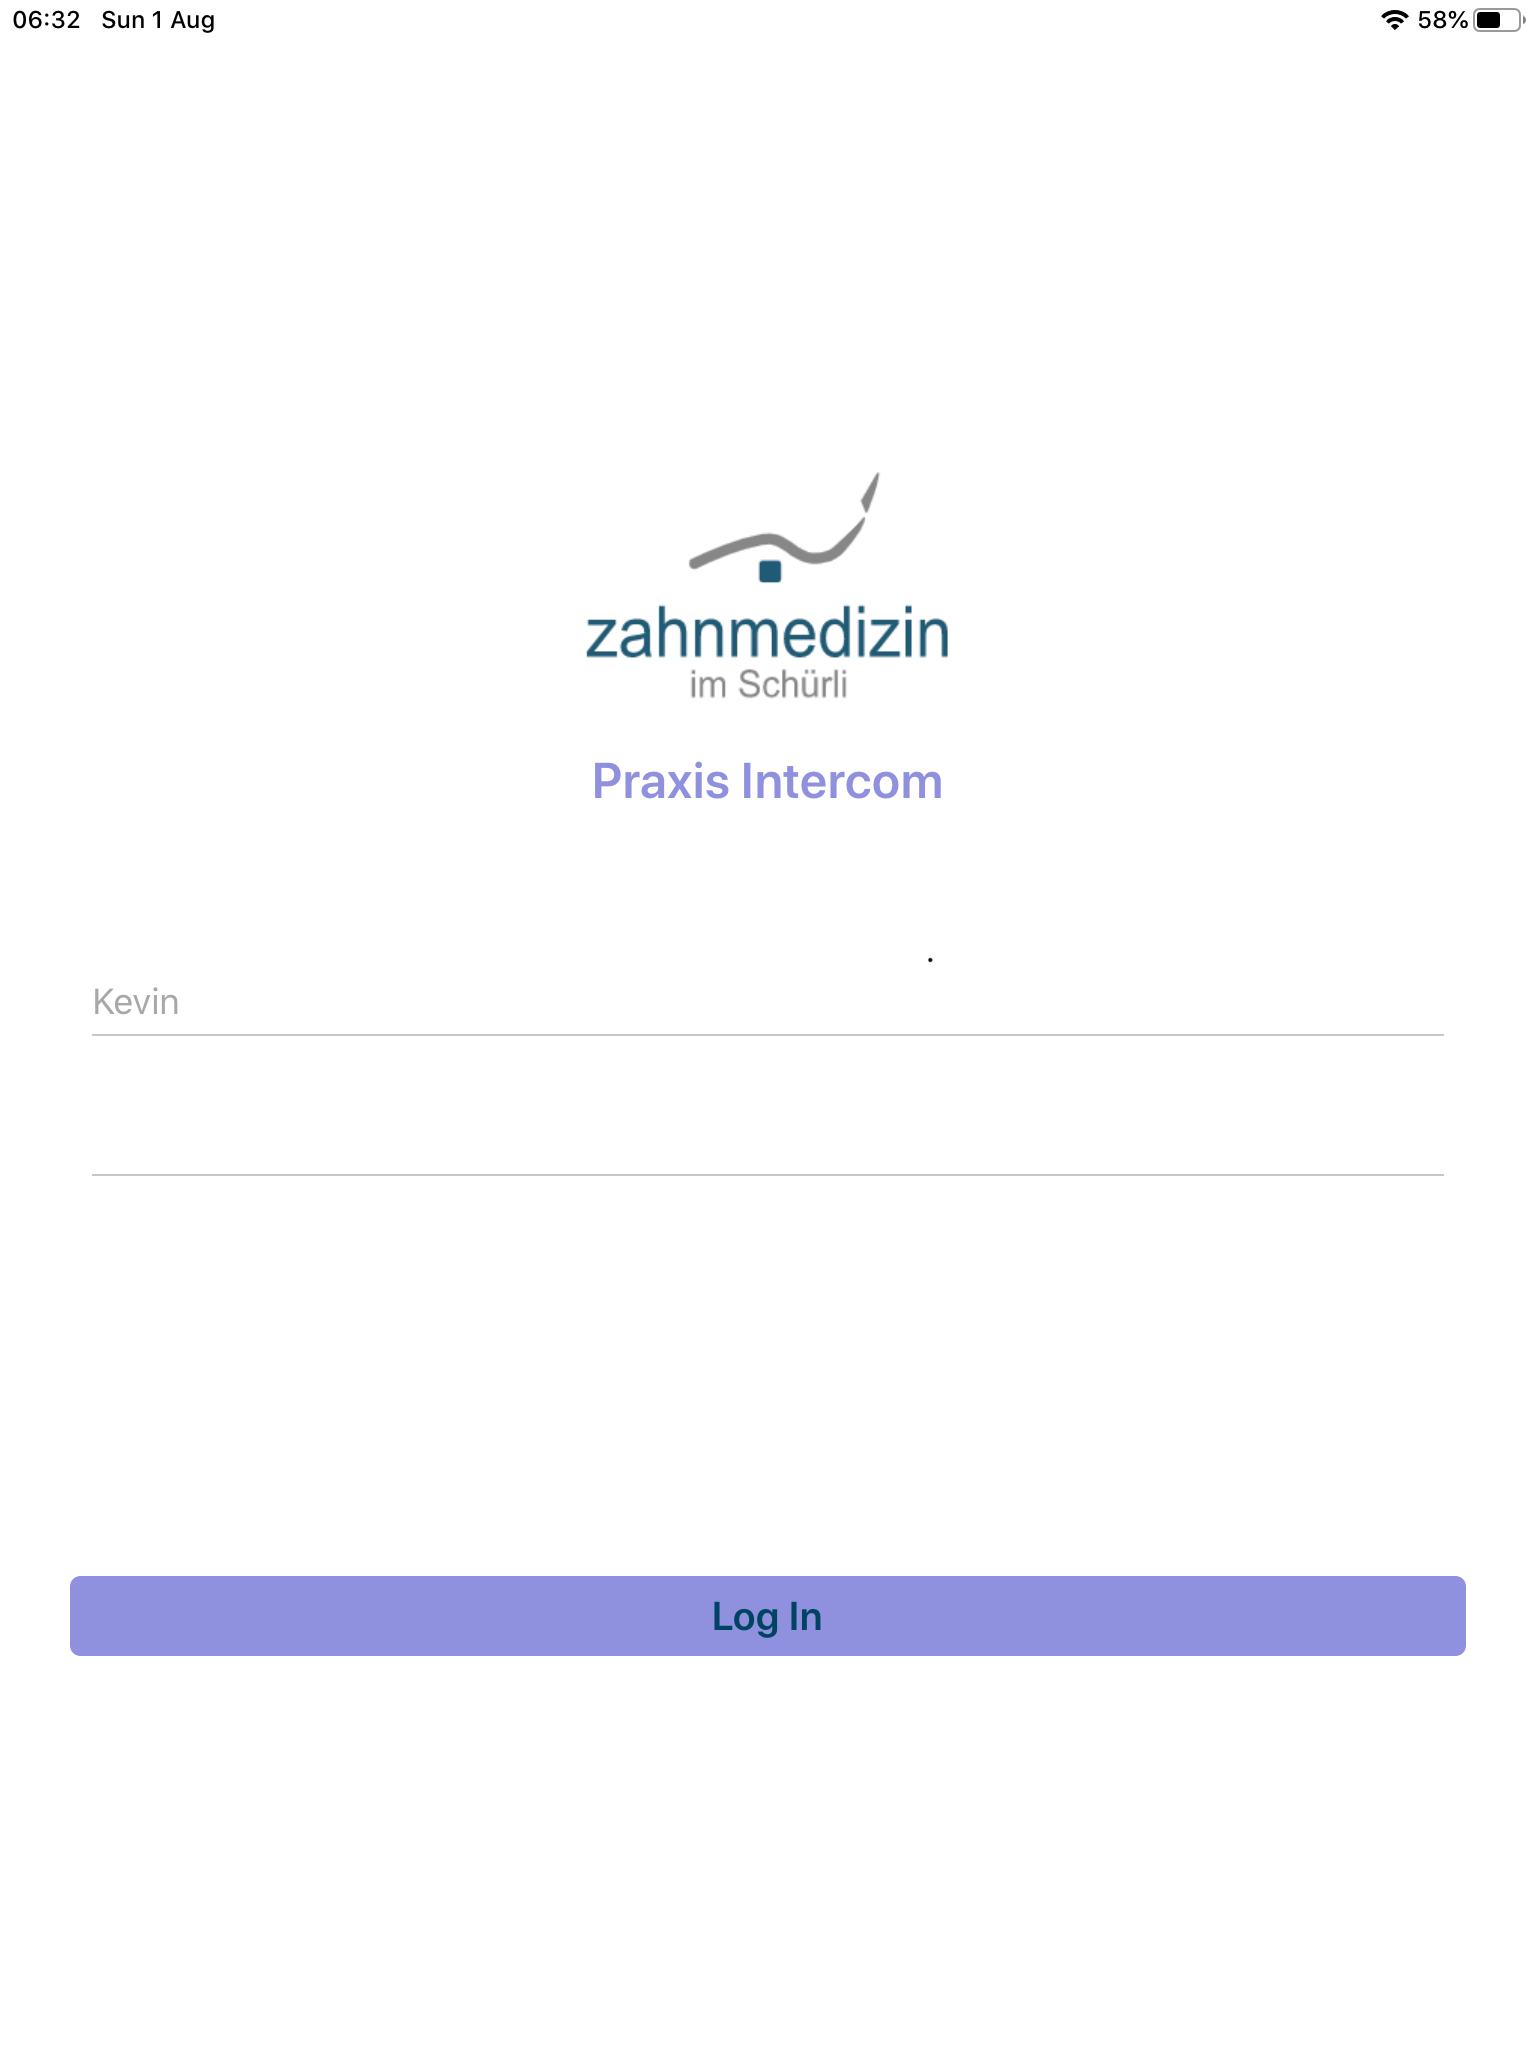
\includegraphics[width=\textwidth]{graphics/screenshots/placeholder}
        \caption{Ansicht Inbox}
    \end{minipage}
    \label{fig:MobileClient-Screens2}
\end{figure}

\clearpage

\subsubsection*{Einstellungen und Aktive Anrufe}

Im Bereich Einstellungen werden Informationen zur gewählten Zimmerkonfiguration und dem angemeldeten Benutzer angezeigt.
Weiter können lokale Einstellungen vorgenommen werden.
Das Vorlesen von empfangenen Benachrichtigungen sowie das Empfangen von Anrufen kann hier deaktiviert werden.
Über einen Button kann der Benutzer sich zudem von der App abmelden.

\begin{figure}[h]
    \centering
    \begin{minipage}[b]{0.4\textwidth}
        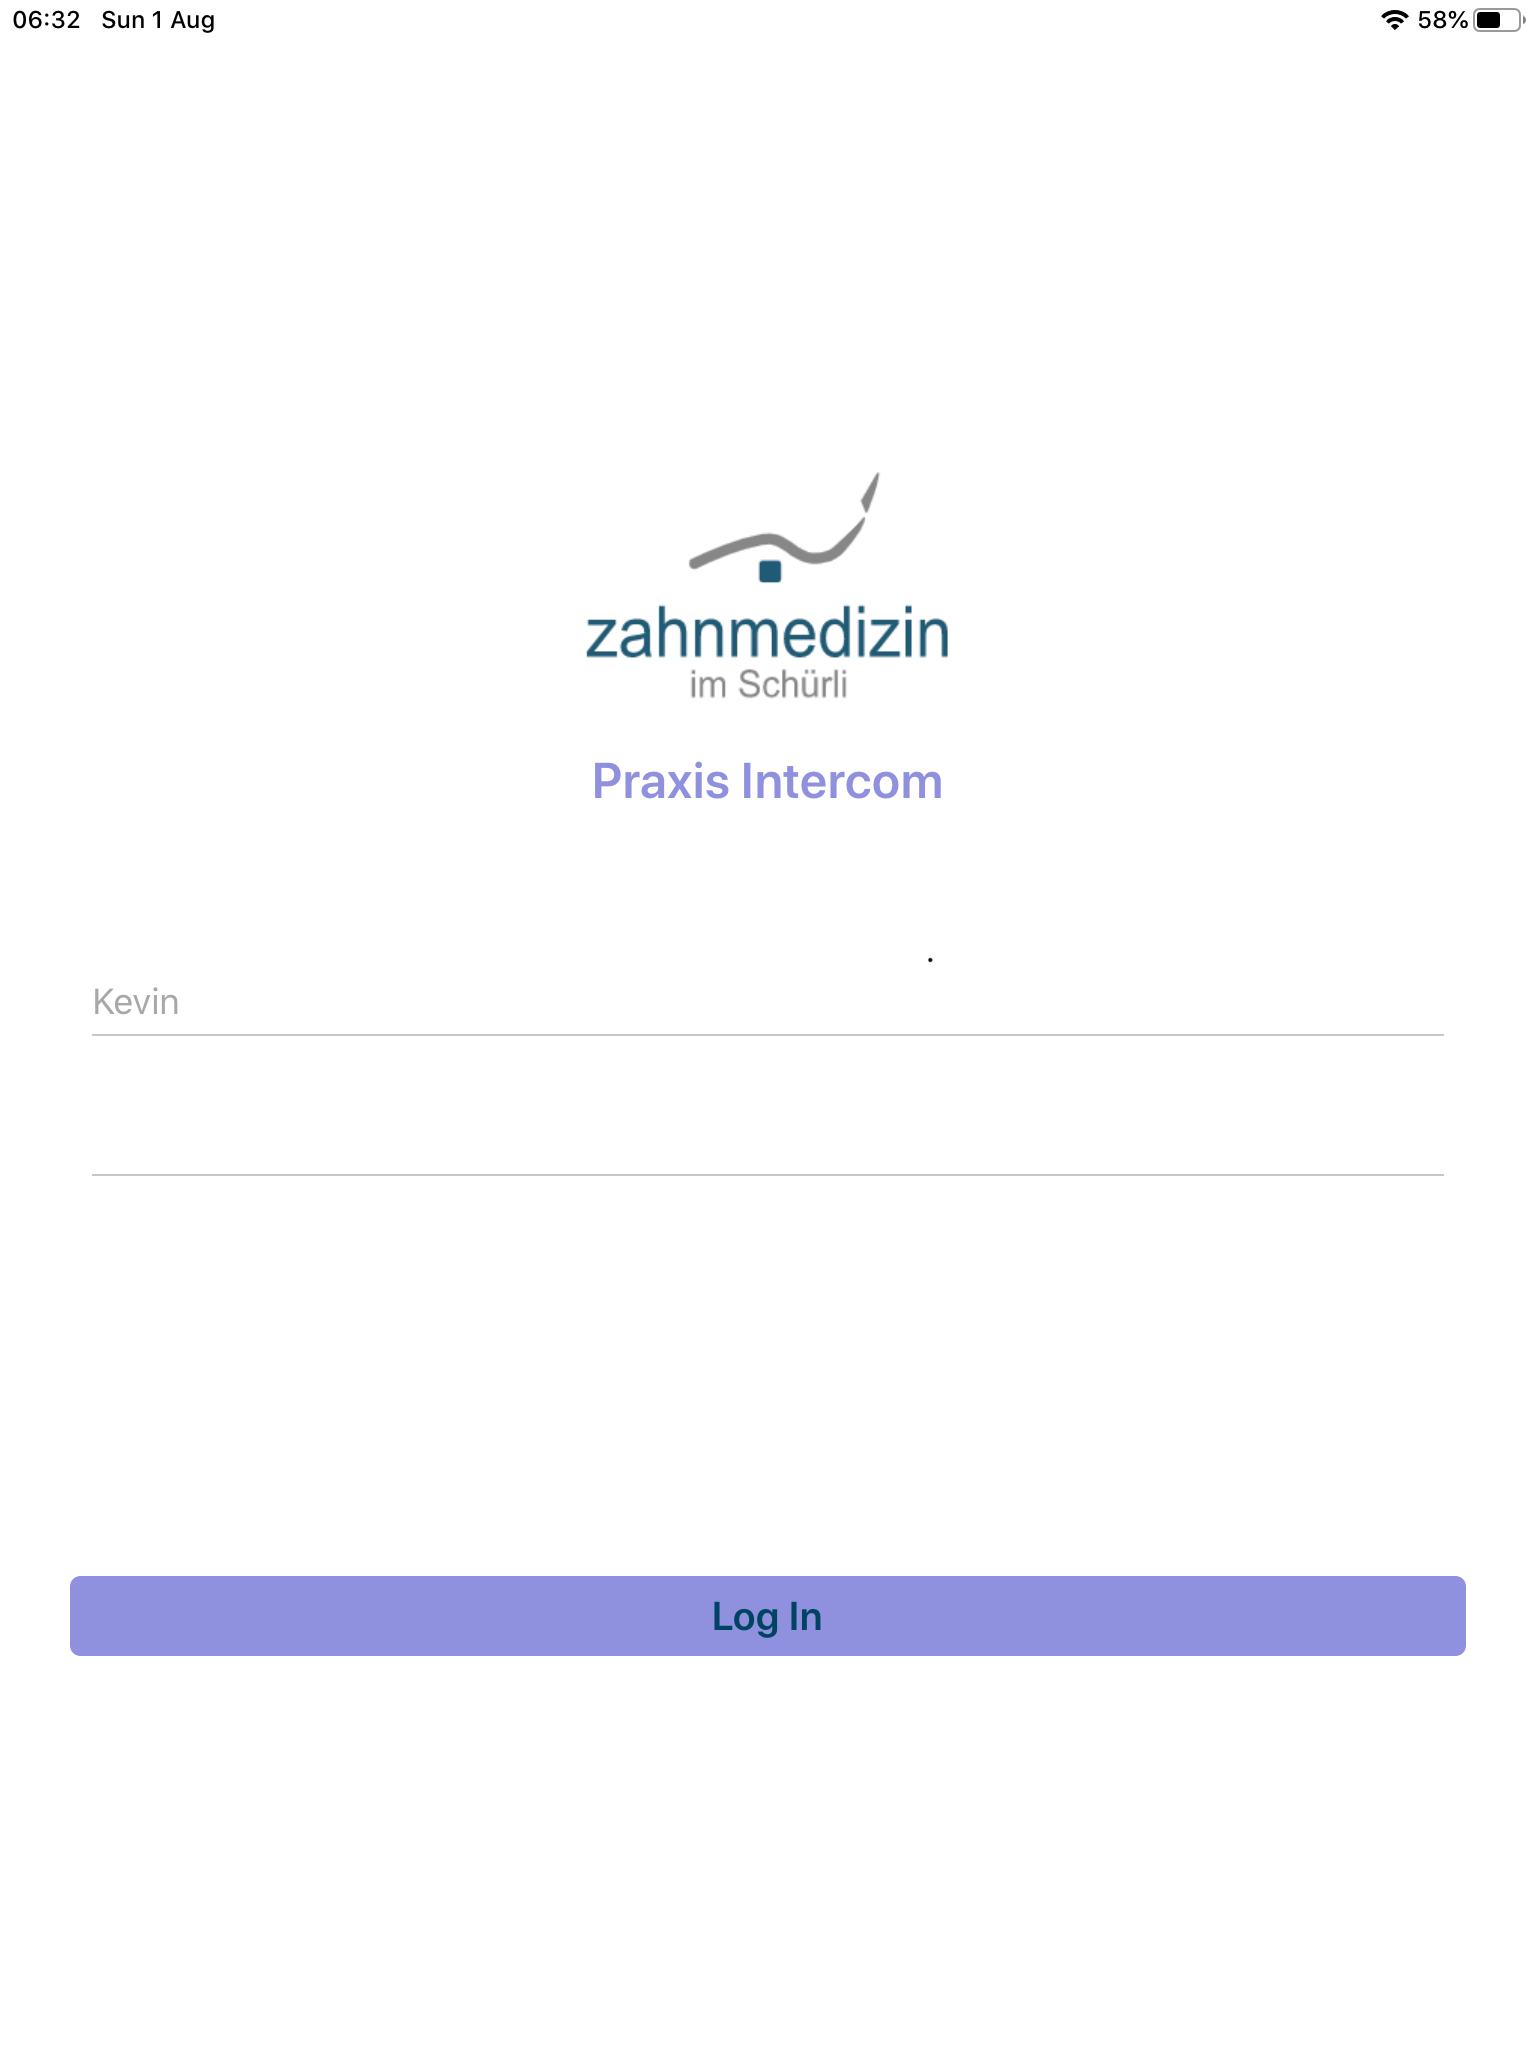
\includegraphics[width=\textwidth]{graphics/screenshots/placeholder}
        \caption{Ansicht Settings}
    \end{minipage}
    \hfill
    \begin{minipage}[b]{0.4\textwidth}
        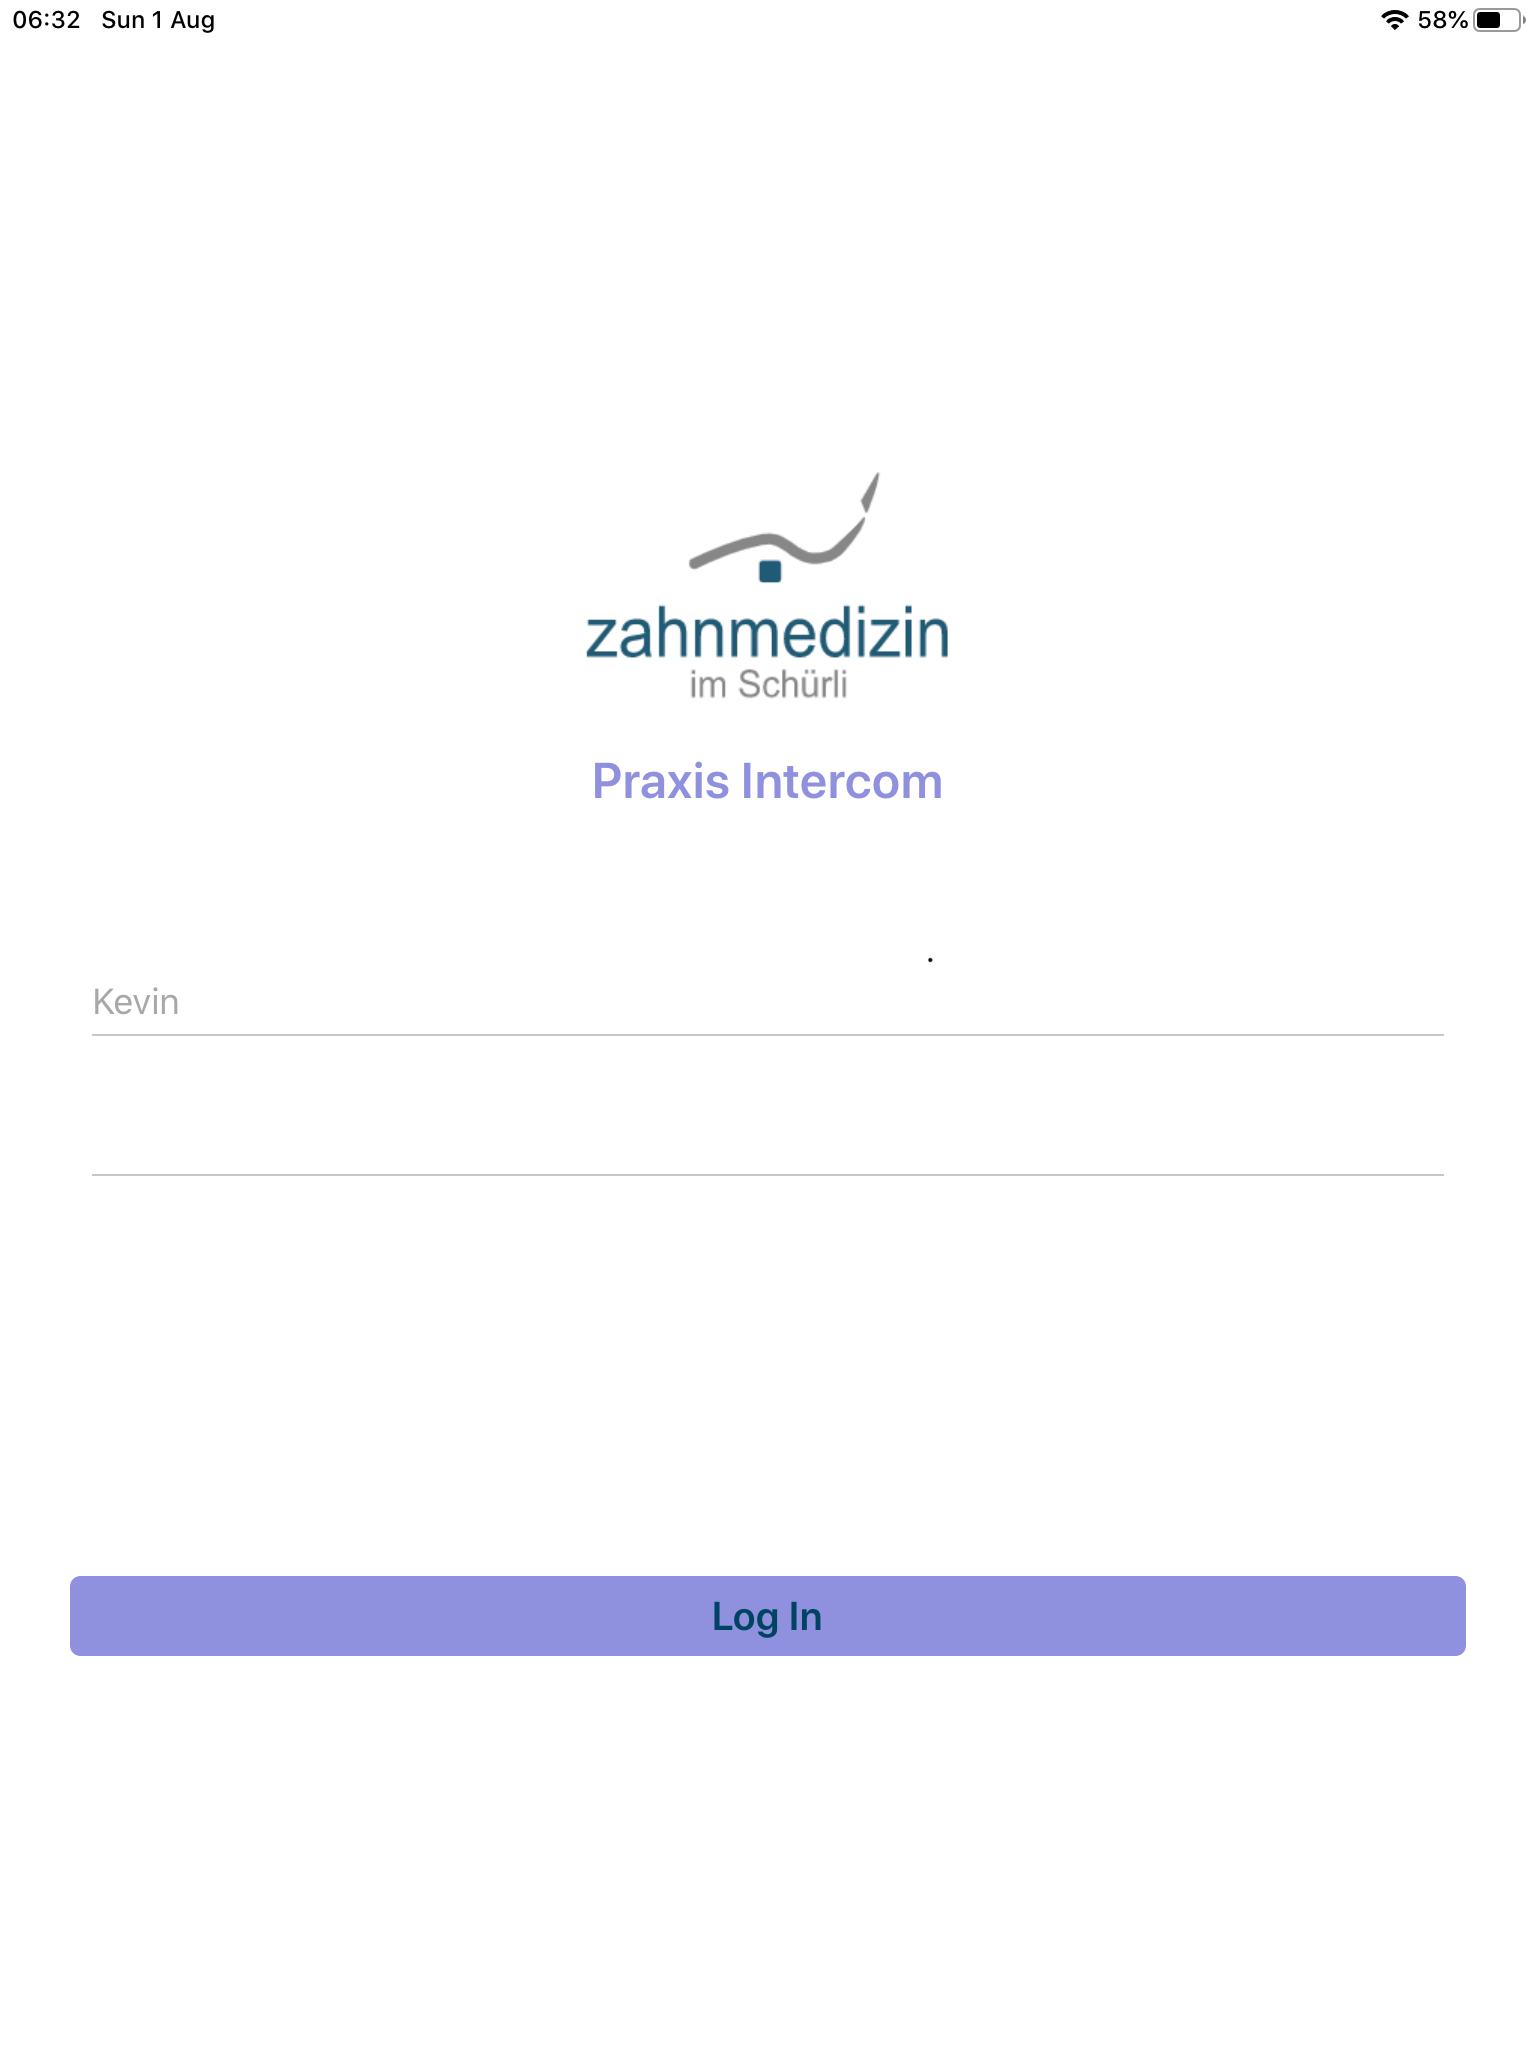
\includegraphics[width=\textwidth]{graphics/screenshots/placeholder}
        \caption{Ansicht Aktiver Anruf}
    \end{minipage}
    \label{fig:MobileClient-Screens3}
\end{figure}

Die Ansicht ''Aktive Anruf'' wird angezeigt, nachdem ein Anruf gestartet wurde.
Entweder, der Anruf durch antippen des Buttons in der Home Ansicht gestartet wurde oder weil ein Anruf von einem anderen Client empfangen wird.
In dieser Ansicht wird der Titel des gestarteten Anrufes bzw. Name des Zimmer des Gesprächspartners angezeigt.
Wenn mehr als ein Gesprächspartner am Anruf beteiligt ist, wird zudem eine Liste der Teilnehmer zusammen mit deren Verbindungsstatus angezeigt.
Allen Gesprächsteilnehmern stehen Buttons zur Stummschaltung des eigenen Lautsprechers und Microphons zur Verfügung.
Zudem können alle Gesprächsteilehmmer die Unterhaltung durch den roten Auflegen Button beenden.

\clearpage

\subsubsection*{Hintergrundbenachrichtigungen und Fehlerhandling}

Das Versenden von Benachrichtigungen ist über die Anbindung des Cloudservices gelöst.
Dieser leitet Benachrichtigungen anhand der Konfiguration über den Messagingservice an die relevanten Empfänger zu.
Bei einem Fehler in der Verarbeitung beim Cloudservice, wird Praxismitarbeitenden direkt mitgeteilt, dass die Benachrichtigung nicht zugestellt werden konnte.
In der App wird ein Dialog angezeigt, welcher darüber informiert und die Möglichkeit bietet, die Aktion direkt zu wiederholen.

\begin{figure}[h]
    \centering
    \begin{minipage}[b]{0.4\textwidth}
        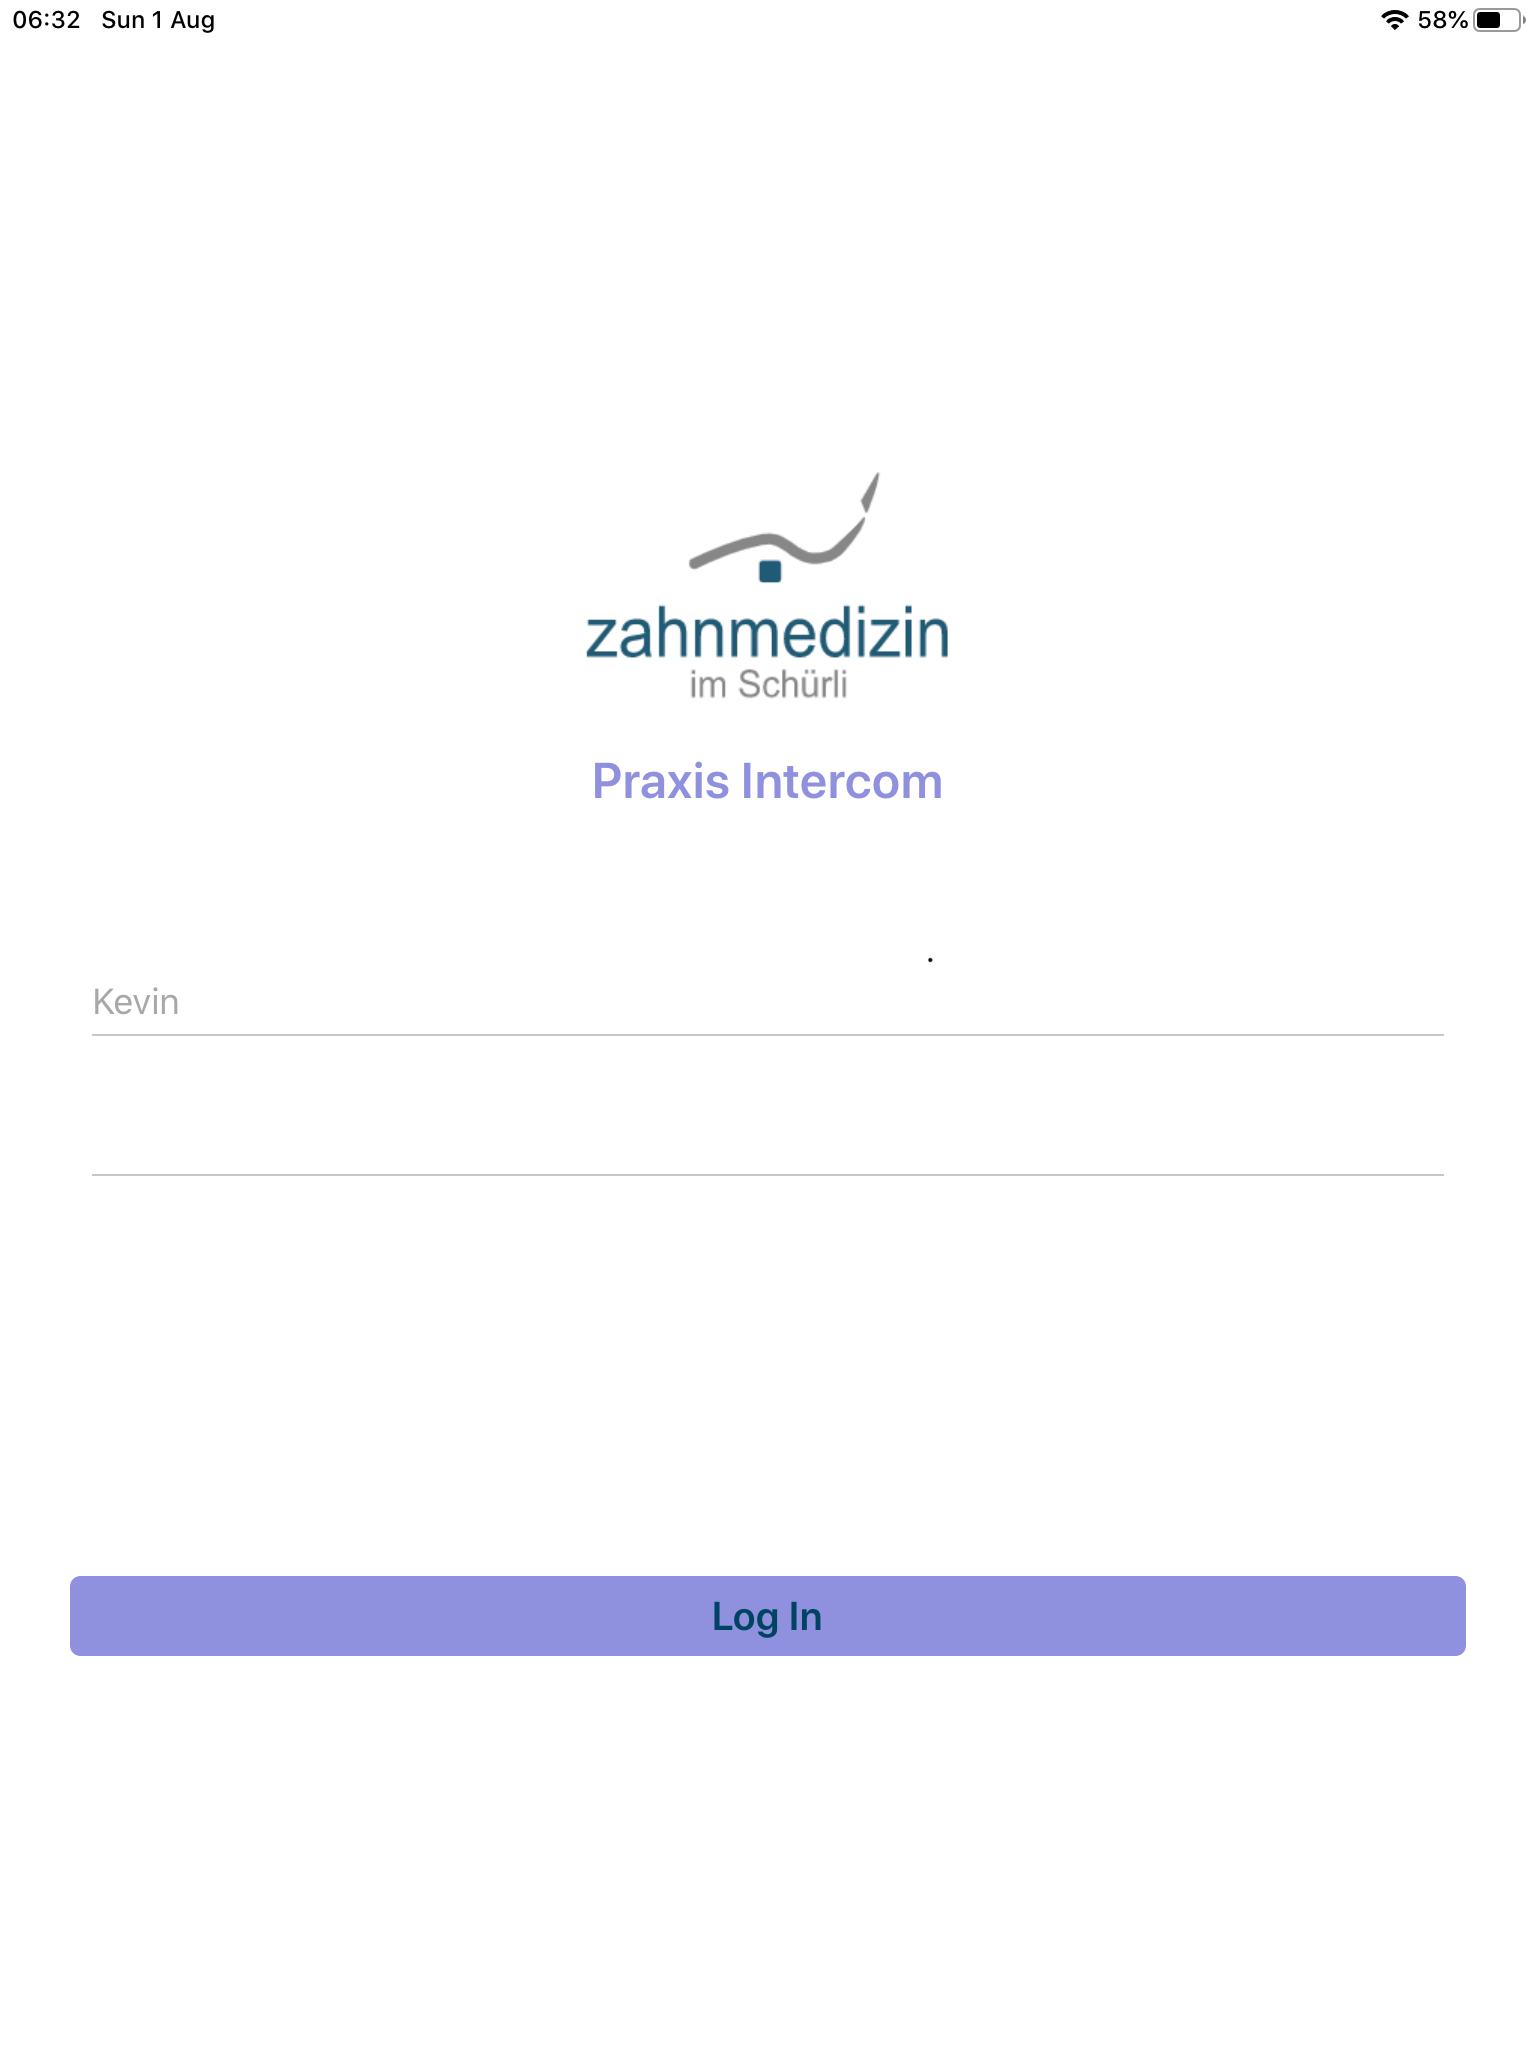
\includegraphics[width=\textwidth]{graphics/screenshots/placeholder}
        \caption{Hintergrund Benachrichtigung}
    \end{minipage}
    \hfill
    \begin{minipage}[b]{0.4\textwidth}
        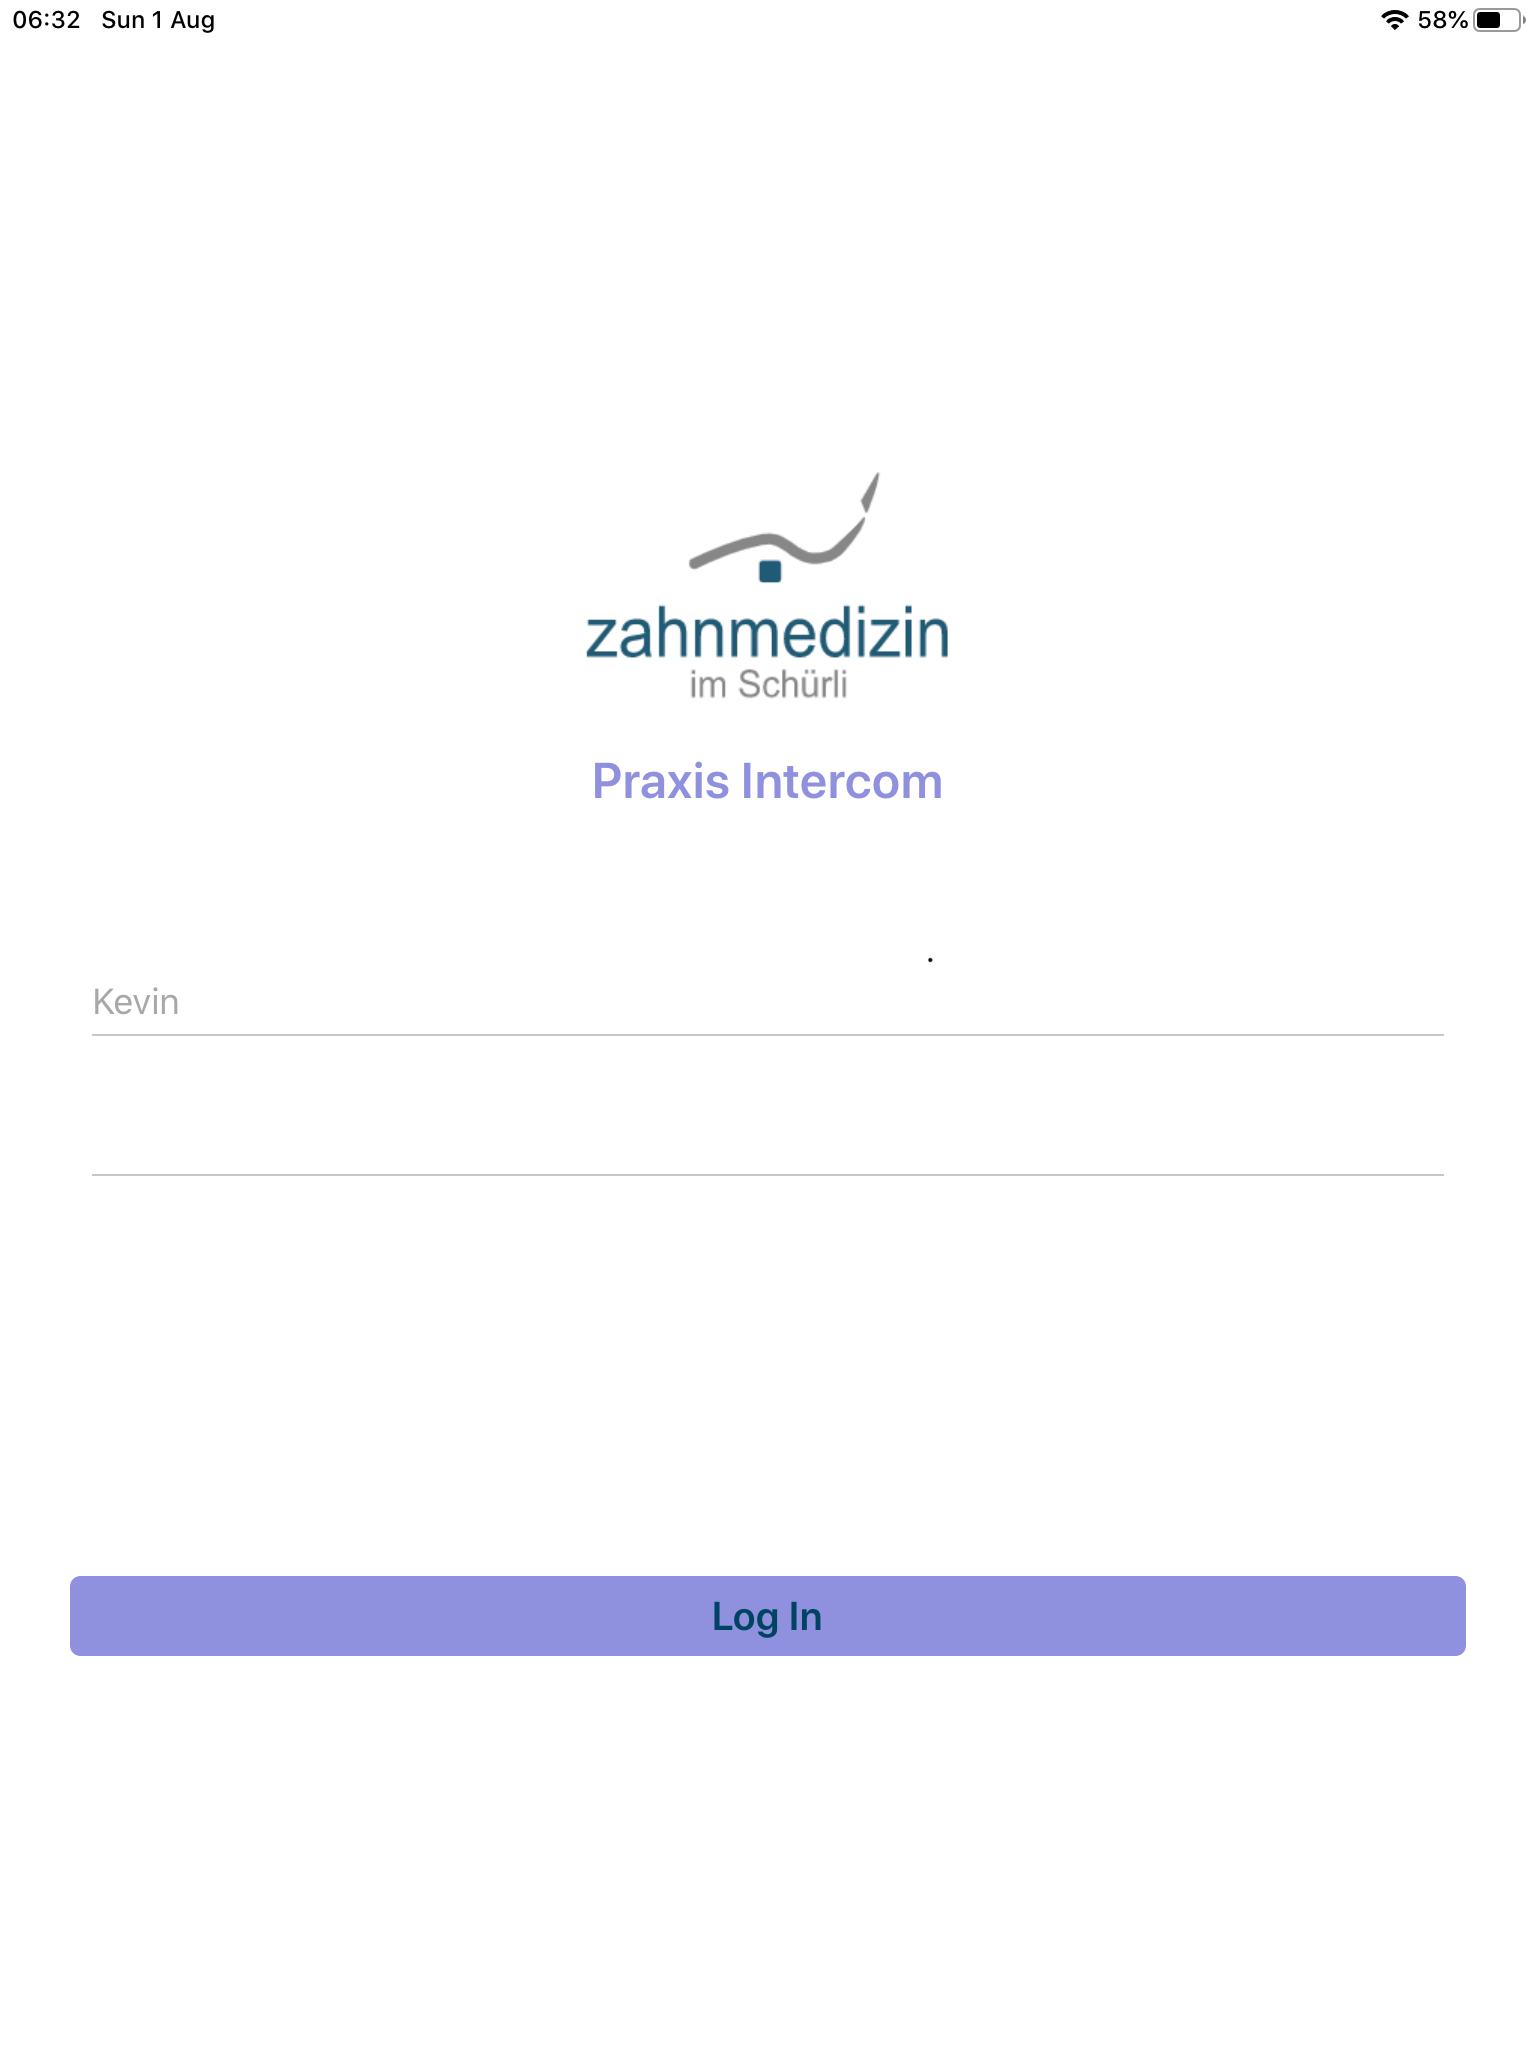
\includegraphics[width=\textwidth]{graphics/screenshots/placeholder}
        \caption{Benachrichtigung wiederholen}
    \end{minipage}
    \label{fig:MobileClient-Screens4}
\end{figure}

Benachrichtigungen können auch im Hintergrund empfangen werden.
Im Hintergrund empfangene Benachrichtigungen erscheinen als Push Benachrichtigungen auf dem Home Screen des iPads.
Anrufe über die Gegensprechanlage können nur empfangen werden, wenn die Applikation geöffnet ist.
Ist die App minimiert oder beendet, ist der jeweilige Client für Gespräche nicht verfügbar.
Ein nicht verfügbarer Client wird über Hintergrundbenachrichtigungen auf verpasste Anrufe hingewiesen.

\clearpage

\subsubsection{Sprachsynthese}

Die Sprachsynthese für Benachrichtigungen in einem Praxisrufsystem konnten vollständig umgesetzt werden.
Praxisadministratoren können über das Admin UI konfigurieren, welche Benachrichtigungen vorgelesen werden.
Beim Empfang einer solchen Benachrichtigung im Mobile Client wird deren Inhalt automatisch vorgelesen.
Die entsprechenden Sprachdaten bezieht der Mobile Client entweder vom Cloudservice oder aus einem lokalen Cache.
Für die Konvertierung von Benachrichtigungen zu Sprachdaten wurde im Cloudservice eine Anbindung an den Sprachsyntheseprovicer AWS Polly implementiert.
Der Cloudservice bietet nach aussen eine Http Schnittstelle über welche Sprachdaten von Benachrichtigungen bezogen werden können.
Sprachdaten müssen immer anhand der technischen Identifikation des relevanten Benachrichtigungstypes angefragt werden.
Die konkreten Daten für die Synthese werden anhand dieser Identifikation aus der persistierten Konfiguration geladen.

\clearpage

\subsubsection{Gegensprechanlage}

Es wurde eine konfigurierbare Gegensprechanlage entwickelt und in Praxisruf integriert.
Die Konfiguration der Gegensprechanlage wurde in die bestehende Konfiguration eingebunden.
Praxisadministratoren können über das Admin UI konfigurieren, welche Sprachverbindungen in welchen Zimmern zu Verfügung stehen.
Diese Konfiguration wird bei der Anmeldung im Mobile Client geladen.
Anhand der Konfiguration werden Buttons für Sprachverbindungen angezeigt.

Praxismitarbeitende können Sprachverbindungen zu anderen Clients über Buttons im Mobile Client starten.
Während laufenden Sprachverbindungen sehen Praxismitarbeitende im Mobile Client den Namen aller Gesprächspartner und deren Verbindungsstatus.
Gesprächsteilnehmende können ihre Sprachverbindungen stummschalten und beenden.
Kann ein Gesprächspartner nicht erreicht werden, wird er mit einer asynchrone Benachrichtigunge über den verpassten Anruf informiert.
Spracherbindungen auf Empfängerseite werden automatisch angenommen.
Bevor die Sprachübertragung aktiviert ist, wird der Empfänger mit einem Benachrichtigungston auf die Verbindung aufmerksam gemacht.
Praxismitarbeitende haben die dieses Verhalten in lokalen Einstellungen anzupassen und Sprachverbindungen zu deaktivieren.
Durch diese Einstellungen, werden Sprachverbindungen immer abgelehnt.
Es wird allerdings eine Benachrichtung angezeigt, welche über den verpassten Anruf informiert.

Sprachverbindungen werden für jeden Gesprächspartner als Peer To Peer Verbindung zwischen Anrufer und Empfänger aufgebaut.
Um diesen Verbindungsaufbau zu ermöglichen, müssen Signale zwischen den Beteiligten ausgetauscht werden.
Dazu wurde der Cloudservice um die Komponente Signaling erweitert.
Diese ermöglicht es Signale über Websocketverbindungen zu versenden.
Sie Signaling Komponenten verwaltet alle offenen Verbindungen und vermittelt Signale an die relevanten Empfänger.
Kann ein Signal nicht zugestellt werden, wird der Empfänger über das Notification Modul mit einer Benachrichtigung informiert.

Die umgesetzte Gegensprechanlage erfüllt alle in Kapitel 3 erarbeiteten Anforderungen.
Sie hat haber zwei Einschränkungen, welche hier erwähnt sein sollen:
Die erste Einschränkung betrifft den Betrieb von Mobile Clients.
Die Qualität der Sprachverbindungen ist ausreichend für eine Gegensprechanlage.
Grundsätzlich ist es möglich, mehrere Endgeräte im selben Zimmer zu betreiben.
Dabei ist aber darauf zu achten, dass diese nicht zu nahe beineinander stehen.
Wird eine Sprachverbindung zwischen zwei Mobile Clients aufgebaut, die unmittelbar nebeneinander stehen kann ein positiver Feedback Loop entstehen, welcher zu einem schrillen Pfeifton führt.
Praxisruf ist für ein Mobile Client pro Zimmer konzipiert.
Diese Einschränkung ist für den Praxisbetrieb minimal bis gar nicht relevant.
Die zweite Einschränkung betrifft den austausch von Sprachdaten.
Sprachverbindungen können zwischen zwei oder mehr Empfängern aufgebaut werden.
Die implementierte Gegensprechanlage hat dabei aber die Einschränkung, dass Verbindungen nur zwischen Anrufer und Empfänger aufgebaut wird.
Es werden keine Verbindungen zwischen den einzelnen Empfängern aufgebaut.
Die implementierte Gegensprechanlage unterstützt damit 1:1 und 1:n Verbindungen aber keine n:n Verbindungen.
